\begin{figure*}[thb!]
  \centering
  \label{fig:approach}
  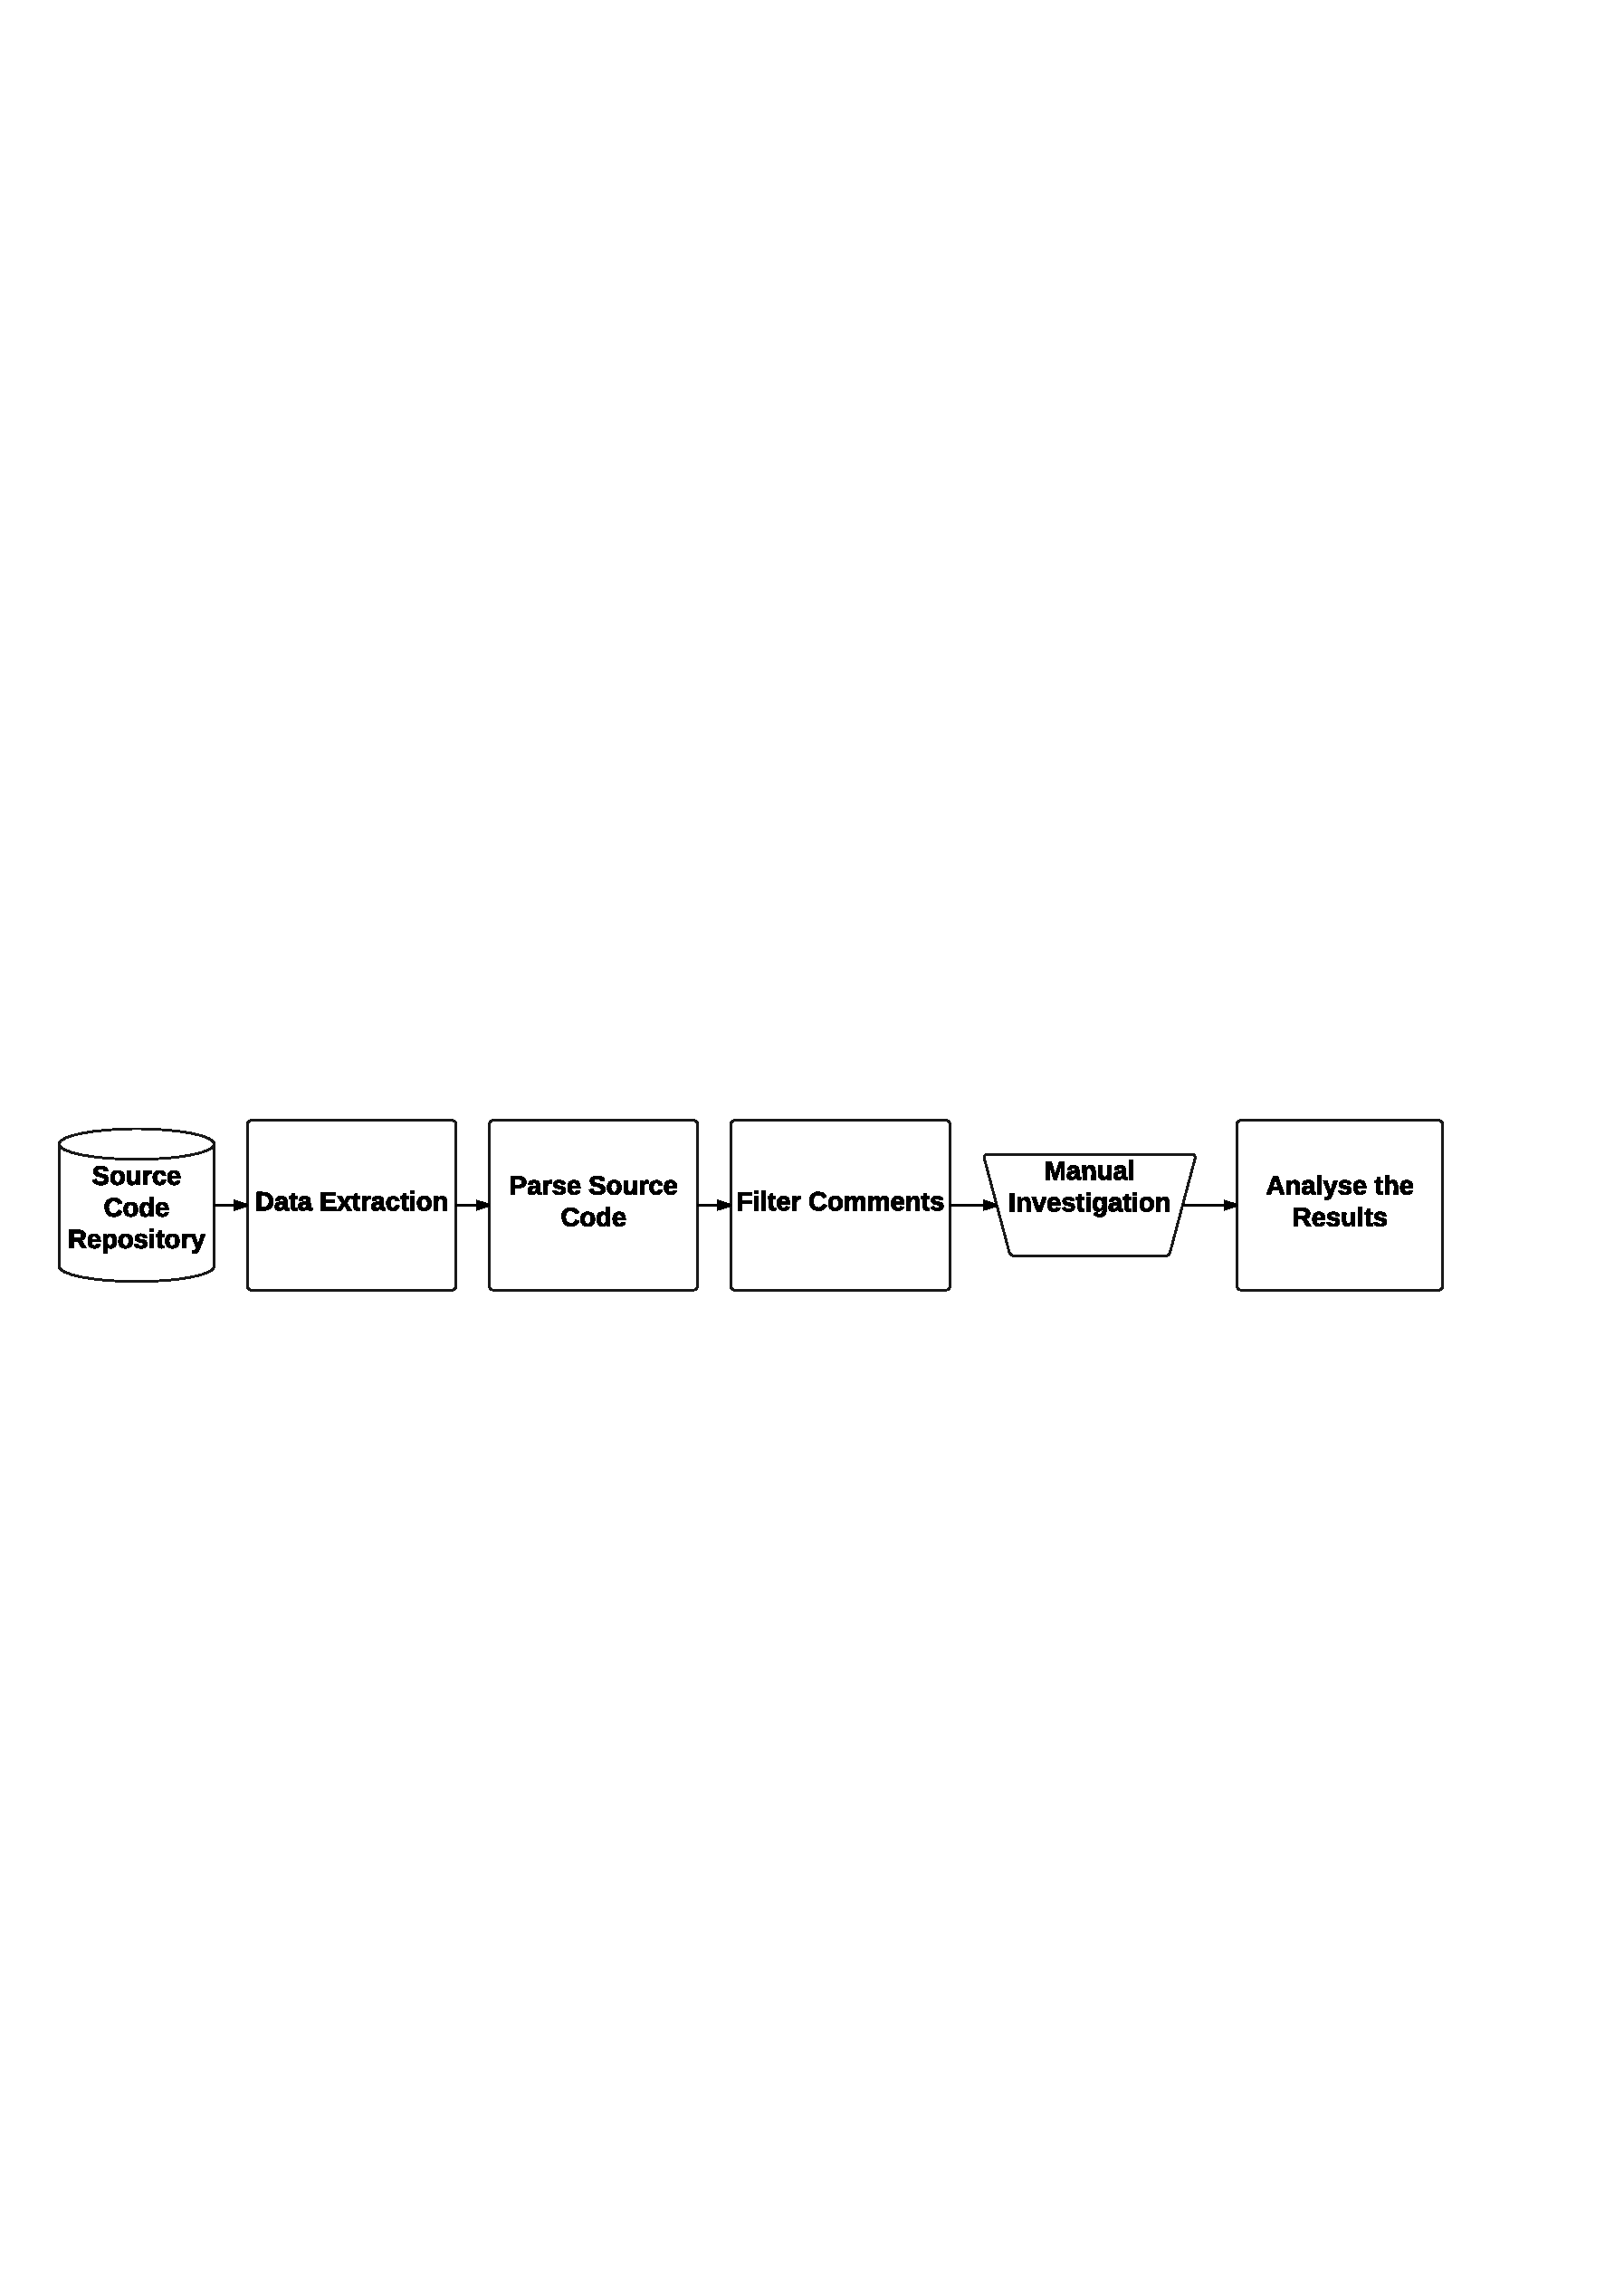
\includegraphics[width=1\textwidth]{figures/Approach}
  \caption{Approach overview}
\end{figure*}

\begin{table*}[!hbt]
      \begin{center}
            \caption{Project Details}
            \label{tab:project_details}
            \begin{tabular}{l| c c c c c }
            \toprule
            \textbf{Project}   & \textbf{Release}  & \textbf{\# of classes}   & \textbf{SLOC}    & \textbf{\# of comments}  & \textbf{\# of contributors} \\ \midrule 
              Apache Ant       & 1.7.0             &  1,475                   & 115,881          & 21,587                   & 70  \\                                   
              Apache Jmeter    & 2.10              &  1,181                   & 81,307           & 20,084                   & 32  \\                                   
              ArgoUML          & 0.34              &  2,609                   & 176,839          & 67,716                   & 87  \\                                   
              Columba          & 1.4               &  1,711                   & 100,200          & 33,895                   & 9   \\                                   
              JFreeChart       & 1.0.19            &  1,065                   & 132,296          & 23,474                   & 18  \\ \bottomrule
            \end{tabular}
      \end{center}
\end{table*}

The main goal of our study is to identify and quantify the different types of self-admitted technical debt found in source code comments. Figure \ref{fig:approach} shows an overview of our approach, and the following subsections detail each step of it.

\subsection{Data Extraction} % (fold)
\label{sub:data_extraction}

To perform our study, we obtain the source code of five open source projects, namely Apache Ant, Apache Jmeter, ArgoUML, Columba and JFreeChart. We chose the aforementioned projects, since they belong to different application domains, and vary in size (e.g., SLOC), and in the number of contributors.

Table \ref{tab:project_details} provides statistics about each one of the projects used in our study. We provide details about the release used, the number of classes, the total source lines of code (SLOC), the total extracted comments and the number of contributors. A source line of code contain at least one valid character, which is not blank spaces or source code comments. In our study, we only use the Java files to calculate the SLOC, and to do so, we use the tool SLOCCount \cite{wheeler2004:home}. 

The number of contributors was extracted from OpenHub, an on-line community and public directory that offers analytics, search services and tools for open source software \cite{Openhub:home}. It is important to notice that the number of comments shown for each project does not represent the number of commented lines, but rather the number of individual line, block, and Javadoc comments. In total, we obtained more than 166,756 comments, found in 8,041 Java classes.
% subsection data_extraction (end)
 
\subsection{Parse Source Code} % (fold)
\label{sub:parse_source_code}
After obtaining the source code of all projects, we extract the comments from their source code. We use JDeodorant \cite{Tsantalis2008CSMR}, an open-source Eclipse plug-in, to parse the source code and extract the code comments. Once extracted, we store all comments in a relational database to facilitate the processing of the data. 
% subsection parse_source_code (end) 

\subsection{Filter Comments} % (fold)
\label{sub:filter_comments}

Source code comments can be used for different purposes in a project like giving context, as part of the documentation, to express thoughts, opinions and authorship, and in some cases, to remove source code from the program. Comments are used freely for developers and with few formalities, if any at all. This informal environment allows developers to bring to light opinions, insights and even confessions (e.g., self-admitted technical debt). 

As shown in prior work by Potdar and Shihab \cite{Potdar2014ICSME}, part of these comments can be identified as self-admitted technical debt, but they are not the majority of cases. With that in mind, we develop and apply 4 filtering heuristics to narrow down the comments eliminating the ones that are less likely to be classified as self-admitted technical debt.

To do so, we developed a Java based tool that reads from the database the data obtained by parsing the source code. Next, it executes the filtering heuristics and stores the result back in the database. The retrieved data contains information like the line number that a class/comment begins/ends and the type, considering the Java syntax, of the comment (i.e., Block, Line or Javadoc). With this information we process the filtering heuristics as described next.

We apply first a heuristic to remove license comments. When license comments are added to the Java files in a project they are generally placed in the first lines of the file, before the class declaration. Based on this knowledge we created a heuristic that eliminates comments that are placed before the class declaration. 

Second, we use a heuristic to merge multiple line comments. Some times developers make long comments, using multiple single-line comments instead of a Block comment. Treating every single line of a long comment as an individual comment causes us to miss important context details that could be recovered by treating all single-line comments as a single block comment. Therefore, we create this heuristic that searches for consecutive single-line comments and groups them.

Third, a heuristic to remove commented source code. Commented source code can be found for many different reasons. One of the possibilities is that the code is not being used, other is that the code is used for debug purposes only. Since commented code does not have self-admitted technical debt, we remove commented source code using a regular expressions that captures typical Java code structures.

Fourth, a heuristic to remove Javadoc comments. The Javadoc comments contain information about the purpose and use of methods and classes. That said, we found that Javadoc comments rarely mention Self-admitted Design Technical Debt. Therefore, we create a heuristic that removes Javadoc comments. To mitigate the risk of eliminating some correct cases, we added one exception - if the comment contains one of the task-reserved words (i.e., ``todo'', ``fixme'', or ``xxx'') we keep that Javadoc comment. We use a simple regular expression to  detect the task-reserved words in the Javadoc comments.

The steps mentioned above significantly reduced the number of comments in our dataset and helped us focus on the most applicable and insightful comments. For example, in the Apache Ant project, applying the above steps helped reduce the number of comments from 21,587 to 4,140 comments meaning that 80.82\% of the comments were filtered. Table \ref{tab:filtering_heuristics_details} provides details for each one of the projects.

\begin{table}[!hbt]
      \begin{center}
            \caption{Filtering heuristics details}
            \label{tab:filtering_heuristics_details}
            \begin{tabular}{l| l l p{1in} }
            \toprule
            \textbf{Project}   & \textbf{\# of comments}  & \textbf{\# after filtering} & \textbf{\%}\\ \midrule 
              Apache Ant       & 21,587                & 4,140                   & 19.17 \% \\ 
              Apache Jmeter    & 20,084                & 8,163                   & 40.64 \% \\
              ArgoUML          & 67,716                & 9,788                   & 14.45 \% \\              
              Columba          & 33,895                & 6,569                   & 19.38 \% \\
              JFreeChart       & 23,474                & 4,436                   & 18.89 \% \\ \bottomrule
            \end{tabular}
      \end{center}
\end{table}
% subsection filter_comments (end)

\subsection{Manual Classification} % (fold)
\label{sub:manual_classification}

To manually classify the comments we first developed a Java based tool that show one comment at time and gives a list of possible classifications  that will be assigned to the comment~\cite{Alves2014MTD}. After applying the different filtering steps, we successfully classified 33,093 comments. The more than 33 thousand comments were classified into five different types of self-admitted technical debt, i.e., design debt, defect debt, documentation debt, requirement debt and test debt.

The first author who made the classification has more than 8 years of experience working in the industry as a software engineer, during this time he designed, implemented and maintained several programs using, in particular the Java programming language. He developed solid skills in object orientated programing and design patterns. We consider that these qualifications provide the necessary background to conduce the manual classification of the comments.   
% subsection manual_classification (end)
